%% GeneDiseaseTrace-LLM: manuscript for the Journal of Biomedical Informatics.
%% Layout and section logic follow a recent JBI paper prepared with elsarticle
%% (Park et al., "Automated Identification of Incidentalomas Requiring Follow-Up", arXiv:2512.05537).
%% Build: latexmk -pdf main.tex
\documentclass[preprint,10pt,letterpaper]{elsarticle}

\usepackage[T1]{fontenc}
\usepackage[utf8]{inputenc}
\usepackage{lmodern}
\usepackage[letterpaper,hmargin=1.35in,vmargin=1.1in]{geometry}   % text block of the model paper
\usepackage{microtype}
\usepackage{amsmath,amssymb}
\usepackage{booktabs,tabularx,multirow,array}
\usepackage{xcolor}
\usepackage{graphicx}
\usepackage[hidelinks]{hyperref}
\usepackage{enumitem}
\setlist{nosep}
\setlength{\emergencystretch}{3em}
\renewcommand{\topfraction}{0.9}
\renewcommand{\floatpagefraction}{0.8}
% Shared palette and TikZ/pgfplots settings for all figures (loaded by main.tex
% and graphical_abstract.tex). Colours are colour-blind safe (Okabe-Ito based).
\usepackage{tikz}
\usepackage{pgfplots}
\pgfplotsset{compat=1.18}
\usepgfplotslibrary{groupplots}
\usetikzlibrary{arrows.meta,positioning,fit,backgrounds,calc,shapes.misc,decorations.pathreplacing}

% Systems
\definecolor{ours}{HTML}{0B5CAD}      % our method (Claude Opus 5.5)
\definecolor{gpt}{HTML}{009E73}       % our method with GPT-6.1 Sol
\definecolor{pubtator}{HTML}{D55E00}  % PubTator3
% Entities
\definecolor{genefill}{HTML}{DCEBFA}
\definecolor{geneline}{HTML}{0B5CAD}
\definecolor{disfill}{HTML}{FBE3D6}
\definecolor{disline}{HTML}{C2410C}
% Statuses
\definecolor{stsup}{HTML}{1B7F4B}
\definecolor{stunc}{HTML}{B45309}
\definecolor{stneg}{HTML}{B4233C}
\definecolor{stnf}{HTML}{475569}
% Neutrals (all text uses dark ink; light tones are for borders/fills only)
\definecolor{ink}{HTML}{1F2933}
\definecolor{rule}{HTML}{CBD5E1}
\definecolor{panel}{HTML}{F8FAFC}

\tikzset{
  panel/.style={draw=rule, fill=panel, rounded corners=3pt, inner sep=6pt},
  paneltitle/.style={font=\sffamily\bfseries\small, text=ink, anchor=north west},
  gene/.style={fill=genefill, draw=geneline, text=ink, rounded corners=1.5pt, inner sep=1.6pt, font=\sffamily\scriptsize},
  dis/.style={fill=disfill, draw=disline, text=ink, rounded corners=1.5pt, inner sep=1.6pt, font=\sffamily\scriptsize},
  badge/.style={rounded corners=2pt, inner sep=1.8pt, font=\sffamily\tiny\bfseries, text=white},
  flow/.style={-{Stealth[length=2.2mm]}, line width=0.9pt, draw=ink},
}
% Inline highlights inside text nodes
\newcommand{\hlgene}[1]{\tikz[baseline=(g.base)]\node[fill=genefill, inner sep=0.6pt, rounded corners=1pt] (g) {\strut #1};}
\newcommand{\hldis}[1]{\tikz[baseline=(d.base)]\node[fill=disfill, inner sep=0.6pt, rounded corners=1pt] (d) {\strut #1};}
\newcommand{\sid}[1]{{\ttfamily\color{ink}\tiny[#1]}}
\newcommand{\badge}[2]{\tikz[baseline=(b.base)]\node[badge, fill=#1] (b) {#2};}

\pgfplotsset{
  gdt/.style={
    font=\sffamily\scriptsize,
    tick label style={font=\sffamily\tiny, text=ink},
    label style={font=\sffamily\scriptsize, text=ink},
    title style={font=\sffamily\bfseries\scriptsize, text=ink, align=center},
    axis line style={draw=ink},
    tick style={draw=ink},
    major grid style={draw=rule, line width=0.3pt},
    grid=major,
  },
}


\newcommand{\st}[1]{\texttt{#1}}             % status and reason-code names
\newcommand{\todo}[1]{\textcolor{stneg}{[TODO: #1]}}

\journal{Journal of Biomedical Informatics}

\begin{document}

\begin{frontmatter}

\title{Evidence-Traceable, Status-Aware Gene--Disease Relation Extraction with a Large Language Model: A Multi-Benchmark Evaluation}

\author[a]{Zeqian Tong}
\author[b]{\todo{co-authors}}
\affiliation[a]{organization={\todo{affiliation}}}
\affiliation[b]{organization={\todo{affiliation}}}

\begin{abstract}
\setlength{\parindent}{0pt}\setlength{\parskip}{6pt}%
\textbf{Objective:} Widely deployed relation extractors such as PubTator3 operate on abstracts and return positive entity pairs without accompanying evidence sentences, certainty grades, or study-versus-background provenance. We developed and evaluated a zero-shot pipeline that extracts gene--disease relations from abstracts and full texts with deterministically grounded sentence citations, a four-way status (\st{supported}, \st{uncertain}, \st{explicit\_negative}, \st{not\_found}), and a source label (this study or background).

\textbf{Methods:} Using one extraction request per paper (and at most one repair request on validation failure), a large language model (Claude Opus 5.5) follows a frozen one-page decision card and cites supporting sentences by ID; a deterministic validator verifies that every entity mention occurs verbatim in the source text and resolves each cited sentence ID to an existing source sentence. Without benchmark-specific tuning, we evaluated the frozen pipeline across BioRED (419 abstracts), EU-ADR (100 abstracts), and 40 RENET2 full-text articles using concept-pair matching, document-level bootstrap confidence intervals, and PubTator3 as comparator.

\textbf{Results:} On BioRED, strict precision was 0.894 and recall was 0.430 (F1 0.581). On a 50-abstract test sample, in-domain PubTator3 achieved higher overall F1 (0.726 vs 0.551); the union of both systems' predictions recovered 73\% of gold relations. On EU-ADR, F1 was comparable (0.506 vs 0.529) and all three negative gold pairs were labelled \st{explicit\_negative}. On RENET2 full texts, our recall exceeded abstract-only PubTator3's (0.370 vs 0.254). Post-hoc routing of stored \st{uncertain} predictions by reason code (selected on BioRED Train+Dev without modifying the prompt) raised held-out Test F1 from 0.542 to 0.627 (recall 0.397 to 0.498) with little change in precision (0.846 vs 0.853) and no extra model calls. Replacing Claude Opus 5.5 with GPT-6.1 Sol yielded a similar F1 (0.555 vs 0.551); extraction with the primary model cost USD 0.056 per abstract and USD 0.44 per full text.

\textbf{Conclusion:} Our pipeline yields precise, syntactically grounded gene--disease extractions that complement supervised tools. Lower recall relative to in-domain classifiers suggests that conservative evidence and entity-scope criteria contribute to the recall gap, a trade-off that users can adjust deterministically at scoring time via the status reason codes.
\end{abstract}

\begin{keyword}
Relation Extraction; Gene--Disease Association; Large Language Models; Biocuration; Evidence Traceability
\end{keyword}

\end{frontmatter}

%% ===================================================================
\section{Introduction}

Curated gene--disease knowledge bases rely on continuous extraction from primary literature. Associations between genes and diseases underpin variant interpretation, drug-target discovery, and structured repositories such as DisGeNET~\cite{pinero2020disgenet} and CTD~\cite{davis2023ctd}. Because more than a million new biomedical articles appear each year, manual curation alone cannot keep pace. Automatic relation extraction has therefore progressed steadily on benchmarks such as BioRED~\cite{luo2022biored}: supervised encoders~\cite{lee2020biobert,gu2021pubmedbert,lai2023biorex} and literature-scale systems such as PubTator3~\cite{wei2024pubtator3} achieve high F1 within their training domain.

Benchmark relation extraction and practical biocuration differ in required output structure and text scope. Widely deployed public extractors such as PubTator3~\cite{wei2024pubtator3} return a flat list of positive pairs from abstracts, whereas biocurators require auditable records across the full paper. First, curators need verbatim supporting sentences to verify each claim quickly. Second, an article may demonstrate an association, hedge it, or report a null result; collapsing these into binary labels discards negative and speculative findings. Third, curators separate a study's primary findings from background literature citations. Finally, abstract-only tools miss relations reported only in the article body: within our 100-paper full-text corpus, 90\% of relations labelled \st{supported} by our pipeline had supporting evidence only outside the abstract.

Large language models can read full papers and follow written rules, but applying them to curation introduces both a reliability problem and an evaluation problem. Brief task prompts leave boundary cases undefined and permit altered quotes or invalid schemas~\cite{chen2025benchmarking,wadhwa2023revisiting}, while multi-turn agent pipelines multiply token costs across repeated calls. Recent full-text evaluations and corpora~\cite{yin2026benchmarking,collins2026biotriplex} extend extraction beyond abstracts, yet they do not deterministically verify cited evidence sentences or provide reason-coded uncertainty grades that let curators adjust recall thresholds after a single run. At the same time, cross-benchmark evaluation is complicated by divergent annotation rules and incomplete gold standards, where unlabelled valid relations are penalized as false positives~\cite{wadhwa2023revisiting,fan2024evaluating}.

We address both challenges in a frozen pipeline requiring one extraction request per paper (with at most one repair request on validation failure). First, a one-page decision card defines explicit entity boundaries, four-way statuses, reason codes, and source labels. Second, a compact line-based output cites supporting sentences by ID only. Third, a deterministic validator guarantees syntactic traceability by rejecting any output whose entity surface forms do not appear verbatim in the paper or whose cited sentence IDs do not resolve to existing source sentences. We evaluate this unchanged pipeline across three benchmarks with distinct annotation protocols (BioRED~\cite{luo2022biored}, EU-ADR~\cite{vanmulligen2012euadr}, and RENET2~\cite{su2021renet2}), compare it with PubTator3~\cite{wei2024pubtator3} and GPT-6.1 Sol, and decompose both missed gold relations and extra predictions outside incomplete gold sets.

%% ===================================================================
\section{Related Work}

\subsection{Supervised Biomedical Relation Extraction}
Supervised domain encoders remain the primary baseline for biomedical relation extraction. Models such as BioBERT~\cite{lee2020biobert} and PubMedBERT~\cite{gu2021pubmedbert} fine-tune pretrained representations on annotated corpora; BioREx~\cite{lai2023biorex} pools heterogeneous datasets to improve generalization (reporting entity-pair relation F1 of 0.74--0.76 on BioRED), and subsequent work incorporates relation directionality~\cite{lai2025directionality}. PubTator3~\cite{wei2024pubtator3} deploys a BioRED-trained extractor alongside entity recognition and normalization modules (reporting 0.86--0.90 F1 on standard gene and disease NER benchmarks) across PubMed and PMC, serving as the standard public resource and our primary comparator. Despite strong in-domain accuracy, these classifiers output binary positive labels without supporting sentences, certainty grades, or provenance, and PubTator3 extracts relations from abstracts only. Our pipeline addresses this curation gap across full texts while complementing supervised candidate recall.

\subsection{Large Language Models for Relation Extraction and Biocuration}
Direct prompting of large language models underperforms supervised encoders on standard relation extraction benchmarks, with zero-shot end-to-end F1 typically ranging between 0.35 and 0.50 on BioRED~\cite{chen2025benchmarking,islamaj2024biocreative,brokman2025benchmark,gade2025benchmarking}. Across the BioCreative VIII BioRED track~\cite{islamaj2024biocreative}, subsequent zero-shot BioRED evaluations~\cite{brokman2025benchmark}, and a survey of 61 biomedical triplet datasets~\cite{gade2025benchmarking}, brief prompts suffered from schema violations, unaligned entity mentions, and inconsistent relation boundaries. Recent studies have benchmarked commercial LLMs on full-text human genetics articles~\cite{yin2026benchmarking}, and structured curation frameworks such as SPIRES (OntoGPT)~\cite{caufield2024spires} and DRAGON-AI~\cite{toro2024dragonai} enforce output templates; however, these approaches rely on short task prompts and emit positive predictions without deterministically verifying cited sentences or grading uncertain and negative claims with actionable reason codes. Our pipeline addresses these limitations through explicit boundary rules, deterministic verification of surface forms and sentence IDs, and reason-coded uncertainty grades.

\subsection{Gene--Disease Benchmarks and Incomplete Gold Standards}
Public gene--disease benchmarks encode different annotation protocols and completeness assumptions. BioRED~\cite{luo2022biored} labels eight relation types between concept pairs in 600 abstracts and marks whether each relation is a primary finding (\emph{Novel}). EU-ADR~\cite{vanmulligen2012euadr} assigns consensus positive, speculative, or negative labels to abstract pairs, where crowdsourced re-annotation has shown that single-annotator positives and guideline boundaries drive many disagreements~\cite{li2015crowdsourcing}. At the full-text level, BioTriplex~\cite{collins2026biotriplex} annotates fine-grained disease--gene relations and provenance across 100 articles split into subsections for supervised fine-tuning, whereas RENET2~\cite{su2021renet2} labels full-text articles at the document level by restricting human review to tool-proposed candidate pairs and assigning negative labels automatically. When generative extractors are scored against selective corpora, unannotated valid relations are counted as false positives alongside factual errors~\cite{wadhwa2023revisiting,fan2024evaluating}. We evaluate one frozen pipeline across BioRED, EU-ADR, and RENET2 without dataset-specific tuning, use stored reason codes and source labels to partition disagreements, and audit explicit negative contradictions separately from uninspected extra predictions.

%% ===================================================================
\section{Methods}

\subsection{Datasets}
Three public benchmarks with distinct annotation protocols and one unlabelled 100-paper PMC corpus evaluate our pipeline across abstracts and full texts (Table~\ref{tab:benchmarks}).

\subsubsection{BioRED}
We used all 419 BioRED abstracts containing at least one gene--disease relation (Train 275, Dev 71, Test 73), totalling 1,633 gold relations. A pair counts as a gold relation when one concept is a gene or gene product and the other is a disease or phenotypic feature, pooled across relation subtypes. We compared against PubTator3 across all 419 abstracts (including the full 73-abstract Test split) and evaluated cross-model consistency with GPT-6.1 Sol on a 50-abstract Test sample. All 419 abstracts were extracted once under the frozen prompt; post-hoc scoring rules for routing stored \st{uncertain} reason codes were selected on Train+Dev only, keeping Test strictly held out.

\subsubsection{EU-ADR}
We evaluated all 100 abstracts of the EU-ADR target--disorder subset, comprising 134 consensus pairs: 122 positive (PA), 9 speculative (SA), and 3 negative (NA). Standard precision and recall treat PA pairs as gold positives, whereas SA and NA pairs evaluate our non-binary status labels.

\subsubsection{RENET2}
We drew a random sample of 40 full-text articles from RENET2 (seed 20261028), whose released texts cover the title, abstract, and early body. This sample contains 181 associated, 83 non-associated, and 1 ambiguous pair; non-associated labels were assigned automatically by text-mining tools without manual verification. Three associated pairs involve an entity absent from the released text and remain in the recall denominator.

\subsubsection{Full-text corpus}
To measure extraction behaviour and cost on complete articles beyond truncated benchmark texts, we ran the pipeline on 100 heterogeneous PMC papers (research articles, case reports, reviews, and one conference-abstract collection) and compared the extracted relations against PubTator3.

\begin{table}[!htbp]
\centering\footnotesize
\caption{\textbf{Public gene--disease benchmarks evaluated in this study.} The three corpora span PubMed abstracts and PMC full texts under different annotation scopes, consensus thresholds, and negative-label protocols.}
\label{tab:benchmarks}
\begin{tabularx}{\linewidth}{@{}l>{\raggedright\arraybackslash}p{2.3cm}>{\raggedright\arraybackslash}X>{\raggedright\arraybackslash}p{3.4cm}>{\raggedright\arraybackslash}p{2.6cm}@{}}
\toprule
Benchmark & Text & Documents used & Gold gene--disease relations & Labels beyond ``related''\\
\midrule
BioRED~\cite{luo2022biored} & PubMed abstracts & 419 abstracts with $\geq$1 gene--disease relation (Train 275 / Dev 71 / Test 73); 50-abstract Test sample & 1,633 & Novel / not novel\\
EU-ADR~\cite{vanmulligen2012euadr} & PubMed abstracts & Target--disorder subset, 100 abstracts & 134 consensus pairs: 122 PA, 9 SA, 3 NA & Positive / speculative / negative\\
RENET2~\cite{su2021renet2} & PMC full text (title, abstract, early body) & Random sample of 40 articles & 181 associated; 83 non-associated; 1 ambiguous & Non-associated labels tool-assigned\\
\bottomrule
\end{tabularx}
\end{table}

\subsection{Relation Extraction}

\subsubsection{Task Definition}
Given one paper as plain text, the extractor identifies primary gene and disease entities, links each entity to all verbatim surface forms in the document, and assigns one of four mutually exclusive statuses to every gene $\times$ disease pair (Table~\ref{tab:status}). Every \st{supported} pair also receives a relation type (causal, correlation, or association) and a source label indicating whether the evidence originates from this study, background citations, both, or is unclear. General symptoms and broad clinical phenotypes are recorded only as auxiliary entities to keep primary disease endpoints specific; Section~\ref{sec:eval} quantifies how this scope boundary affects benchmark recall.

\begin{table}[!htbp]
\centering\footnotesize
\caption{\textbf{Four-way pair status schema assigned to every extracted gene $\times$ disease pair.} Only \st{supported} pairs count as positive predictions under the default strict evaluation view; \st{uncertain} pairs require one or more explicit reason codes.}
\label{tab:status}
\begin{tabularx}{\linewidth}{@{}lX@{}}
\toprule
Status & Definition\\
\midrule
\textcolor{stsup}{\st{supported}} & The text reports a finding or an explicit attribution linking the pair (not an aim or a hypothesis), and the link is readable in the text.\\
\textcolor{stunc}{\st{uncertain}} & There is potential evidence, but hedging, scope, identity, co-reference, presupposition or a conflict prevents a decision. A reason code is required.\\
\textcolor{stneg}{\st{explicit\_negative}} & The text explicitly reports no association, or an opposite result, for this pair on a stated question.\\
\textcolor{ink}{\st{not\_found}} & Everything else, including co-occurrence only. It does not mean the pair is medically unrelated.\\
\bottomrule
\end{tabularx}
\end{table}

\subsubsection{Decision Card}
A frozen one-page decision card governs all entity and relation judgments across benchmarks. Prior to any benchmark evaluation, we manually annotated three pilot full-text articles and audited cross-model disagreements to formulate a 20,000-token annotation guideline comprising 16 rules (R1--R16) and 35 boundary cases. We then distilled this guideline into a 1,000-word decision card paired with a 600-word output format specification. The card defines entity typing and merging, the four pair statuses, relation types, source labels, and explicit boundary rules: sentence co-occurrence alone is never a relation; authors' hedged statements receive status \st{uncertain} with reason code \st{hedged\_claim}; genetic variants described without disease attribution are excluded; and statistical tests support a pair only when they directly test that gene against that disease outcome. This card was frozen as variant V1 before any benchmark run and was applied unchanged during extraction across all datasets; benchmark splits were used only at evaluation time to select post-hoc operating points over stored outputs (Section~\ref{sec:eval}).

Boundary-case checks and development comparisons on 12 held-out stratified full-text papers (excluding the three pilot articles) established the prompt format and reasoning configuration before freezing V1. Across three runs on the 35 boundary cases, the 1,000-word card matched the full 20,000-token guideline on 110 of 112 decision checks; across the 12 full-text papers, condensing the full guideline into the one-page card (V1 vs V2) preserved extraction behaviour, reaching 0.976 pair-status agreement while reducing first-request cost by about 12\%. Lowering reasoning effort from medium to low (V3) cut cost by 24\% but missed about 10\% of genes, diseases, and supported relations; we therefore fixed medium reasoning effort for all experiments. Because these development runs varied prompt length and reasoning effort within the same structured pipeline, isolating the specific causal effect of the decision card requires a minimal-prompt baseline without the card (Section~\ref{sec:limitations}).

\subsubsection{Extraction Pipeline}
Every paper passes through four sequential steps: deterministic packing, language-model generation, deterministic expansion, and schema validation (Fig.~\ref{fig:pipeline}). First, in \emph{Packing}, deterministic code splits the document into numbered blocks and sentences with stable IDs (e.g.\ \texttt{b0012.s3}), strips the reference section, and places the frozen decision card and format specification into a cached system prompt. Second, in \emph{Generation}, one extraction request to Claude Opus 5.5 (medium reasoning effort, all tools disabled) emits pipe-separated lines encoding entities, evidence items, pair judgments, study findings, conflicts, and rule gaps; the model cites evidence by sentence ID only, preventing altered quotations and reducing output tokens. Third, in \emph{Expansion}, a deterministic script matches every predicted surface form verbatim in the text, resolves sentence IDs to exact quotes and character offsets, and completes the full gene $\times$ disease matrix by filling unlisted pairs as \st{not\_found}. Fourth, in \emph{Validation}, a deterministic validator checks that every surface form occurs verbatim, every cited sentence ID resolves to an existing source sentence, pair endpoints are primary entities, and all \st{uncertain} pairs carry valid reason codes. This validation step guarantees verbatim entity grounding, valid sentence-ID resolution, and schema compliance; semantic judgment of whether a cited sentence supports the relation remains with the language model under the decision card. Any validation error triggers at most one repair request listing the exact violations. Across the 100-paper full-text corpus, 69 papers passed on the first request and 31 required one repair; all 100 passed after repair, with every repair fixing formatting without changing substantive pair judgments. Fig.~\ref{fig:example} shows the complete pipeline output on one full-text article.

\begin{figure}[!htbp]
\centering
\resizebox{\linewidth}{!}{% Figure 1 in the manuscript. Four-step extraction pipeline with concise keyword nodes and dark ink text.
\newcommand{\stagebox}[2]{\begin{minipage}[t][2.25cm][t]{#1}\raggedright #2\end{minipage}}
\newcommand{\codeline}{\ttfamily\fontsize{6.4pt}{7.6pt}\selectfont\color{ink}}
\begin{tikzpicture}[
  font=\sffamily\scriptsize, text=ink,
  every node/.append style={execute at begin node={\hyphenpenalty=10000\exhyphenpenalty=10000}},
  stage/.style={draw=rule, fill=panel, rounded corners=3pt, align=left, inner sep=4.5pt, anchor=north west},
  llm/.style={stage, draw=ours, fill=genefill, line width=0.8pt},
  io/.style={draw=rule, fill=white, rounded corners=2pt, text width=1.85cm, align=left, inner sep=3.5pt},
  note/.style={font=\sffamily\scriptsize, text=ink},
]
% Steps (top-aligned, equal height, keyword-only)
\node[stage] (pack) at (2.75,0) {\stagebox{2.2cm}{%
  {\bfseries 1\enspace Packing}\par\smallskip
  Assign sentence IDs\par
  Drop references\par
  Cache system prompt\par\smallskip
  {\codeline b0098.s12}}};
\node[llm] (gen) at ($(pack.north east)+(0.45,0)$) {\stagebox{2.65cm}{%
  {\bfseries\color{ours} 2\enspace LLM Generation}\par\smallskip
  One extraction call\par
  Cite sentence IDs only\par\smallskip
  {\codeline E|G5|gene|MAP3K3|...\\EV|V7|b0098.s12|...\\P|G5|D3|sup|a|bg|...}}};
\node[stage] (exp) at ($(gen.north east)+(0.45,0)$) {\stagebox{2.2cm}{%
  {\bfseries 3\enspace Expansion}\par\smallskip
  Match surface forms\par
  Resolve quotes \& offsets\par
  Fill gene $\times$ disease matrix}};
\node[stage] (val) at ($(exp.north east)+(0.45,0)$) {\stagebox{2.2cm}{%
  {\bfseries 4\enspace Validation}\par\smallskip
  Verify verbatim spans\par
  Verify sentence IDs\par
  Check schema \& reasons}};
% Inputs and output, centred on the step row
\path (pack.west) ++(-0.45,0) coordinate (inmid);
\node[io, anchor=south east] (paper) at ($(inmid)+(0,0.08)$) {\textbf{Paper}\\Full text or abstract};
\node[io, anchor=north east] (card) at ($(inmid)+(0,-0.08)$) {\textbf{Decision card}\\Frozen rules + schema};
\node[io, anchor=west] (out) at ($(val.east)+(0.6,0)$) {\textbf{Output}\\Entities \& mentions\\Evidence quotes\\4-status pair matrix};
% Arrows
\draw[flow] (paper.east) -- ++(0.2,0) |- ([yshift=3pt]pack.west);
\draw[flow] (card.east) -- ++(0.2,0) |- ([yshift=-3pt]pack.west);
\draw[flow] (pack) -- (gen);
\draw[flow] (gen) -- (exp);
\draw[flow] (exp) -- (val);
\draw[flow, draw=stsup] (val) -- node[above, note, text=stsup, font=\sffamily\scriptsize\bfseries] {pass} (out);
% Repair loop below the row
\draw[flow, draw=stneg, densely dashed, line width=1pt] (val.south) -- ++(0,-0.42) -| (gen.south);
\node[note, text=stneg, anchor=north, align=center] (fail) at ($(gen.south)!0.5!(val.south)+(0,-0.48)$)
  {\textbf{fail} $\rightarrow$ at most 1 repair request with error list};
% Legend on the left
\node[note, anchor=north west, text=ink] (leg) at ($(card.west |- fail.south)+(0,0.18)$)
  {\textcolor{ours}{\rule{7pt}{7pt}}\,LLM call\quad \textcolor{rule!80!black}{\rule{7pt}{7pt}}\,Deterministic code};
\end{tikzpicture}
}
\caption{\textbf{Architecture of the four-step extraction pipeline.} Steps~1, 3, and~4 execute deterministic code; Step~2 makes one extraction request to the language model. Any output that fails verbatim surface-form, sentence-ID, or schema checks in Step~4 triggers at most one repair request listing the exact validation errors.}
\label{fig:pipeline}
\end{figure}

\begin{figure}[!htbp]
\centering
\resizebox{\linewidth}{!}{% Figure 2. Worked example: PMC10014009 (Kim et al., 2023; CC BY-NC-ND 4.0, short quotes).
\newcommand{\fG}[1]{{\setlength{\fboxsep}{0.8pt}\colorbox{genefill}{\strut\textcolor{geneline!85!black}{#1}}}}
\newcommand{\fD}[1]{{\setlength{\fboxsep}{0.8pt}\colorbox{disfill}{\strut\textcolor{disline!85!black}{#1}}}}
\newcommand{\fS}[1]{\leavevmode{\ttfamily\tiny\color{ink}#1}}
\newcommand{\fst}[2]{\leavevmode{\setlength{\fboxsep}{1.2pt}\colorbox{#1}{\textcolor{white}{\sffamily\tiny\bfseries #2}}}}
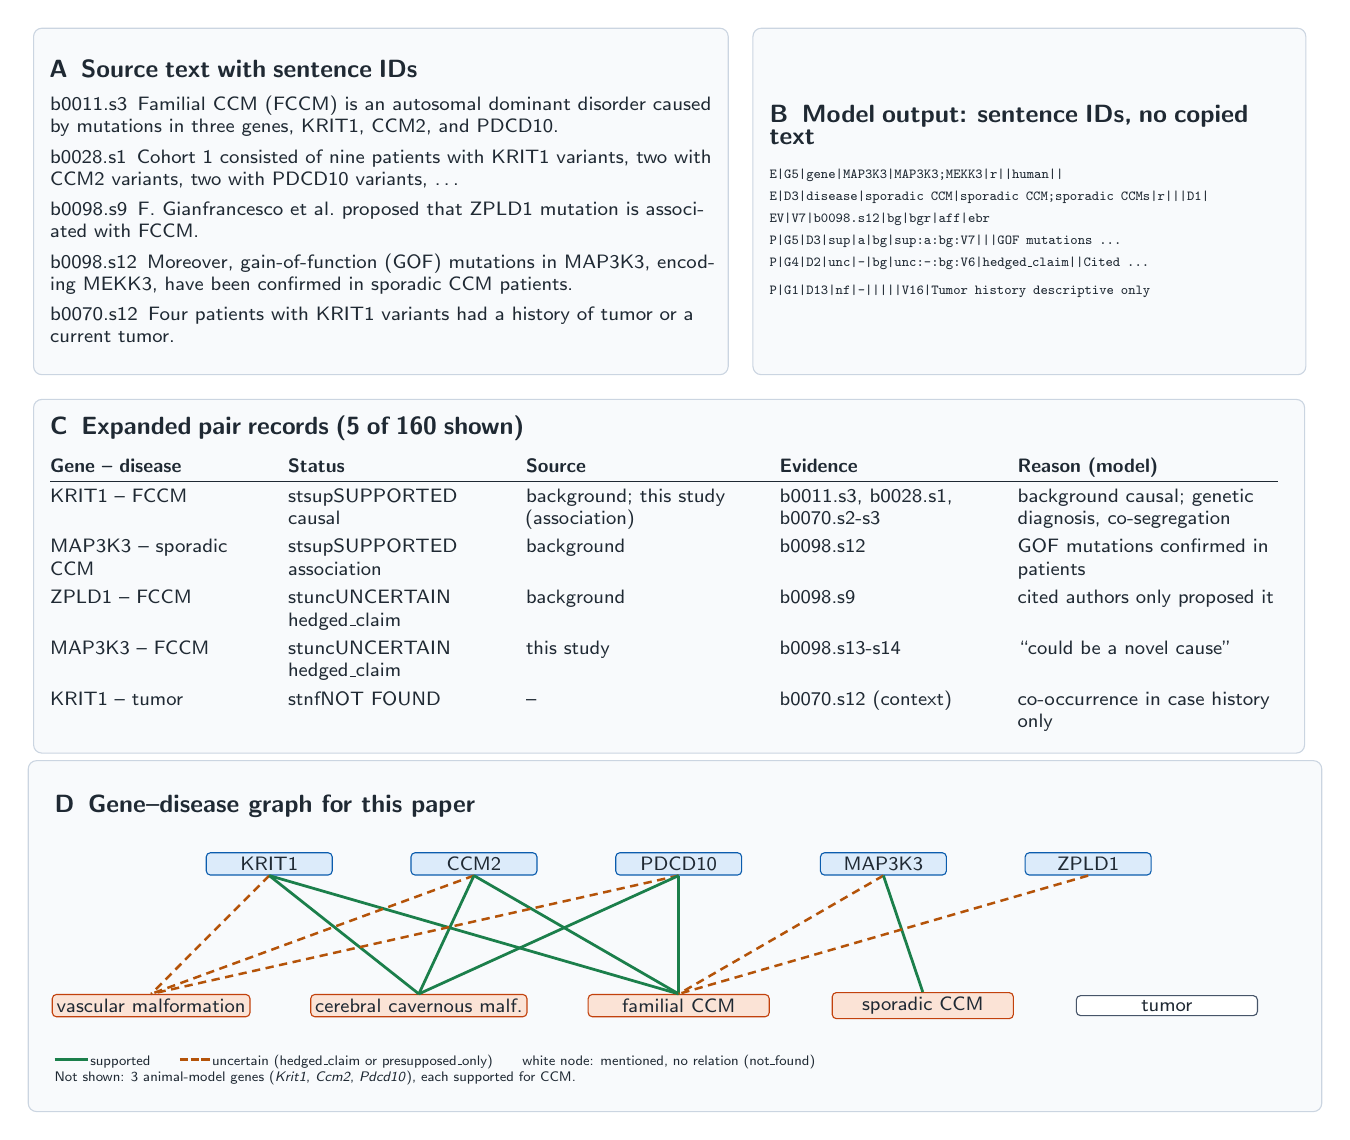
\begin{tikzpicture}[font=\sffamily\scriptsize, text=ink]
% ---------------- Panel A: source text
\node[panel, text width=8.4cm, minimum height=4.4cm, align=left, anchor=north west] (A) at (0,0) {%
  {\sffamily\bfseries\small A\enspace Source text with sentence IDs}\\[4pt]
  \fS{b0011.s3}\enspace \fD{Familial CCM (FCCM)} is an autosomal dominant disorder caused by mutations in three genes, \fG{KRIT1}, \fG{CCM2}, and \fG{PDCD10}.\\[3pt]
  \fS{b0028.s1}\enspace Cohort 1 consisted of nine patients with \fG{KRIT1} variants, two with \fG{CCM2} variants, two with \fG{PDCD10} variants, \dots\\[3pt]
  \fS{b0098.s9}\enspace F. Gianfrancesco et al.\ proposed that \fG{ZPLD1} mutation is associated with \fD{FCCM}.\\[3pt]
  \fS{b0098.s12}\enspace Moreover, gain-of-function (GOF) mutations in \fG{MAP3K3}, encoding \fG{MEKK3}, have been confirmed in \fD{sporadic CCM} patients.\\[3pt]
  \fS{b0070.s12}\enspace Four patients with \fG{KRIT1} variants had a history of \fD{tumor} or a current \fD{tumor}.};
% ---------------- Panel B: model output
\node[panel, text width=6.6cm, minimum height=4.4cm, align=left, anchor=north west] (B) at ($(A.north east)+(0.3,0)$) {%
  {\sffamily\bfseries\small B\enspace Model output: sentence IDs, no copied text}\\[6pt]
  {\ttfamily\tiny\color{ink}%
  E|G5|gene|MAP3K3|MAP3K3;MEKK3|r||human||\\[2pt]
  E|D3|disease|sporadic CCM|sporadic CCM;sporadic CCMs|r|||D1|\\[2pt]
  EV|V7|b0098.s12|bg|bgr|aff|ebr\\[2pt]
  P|G5|D3|sup|a|bg|sup:a:bg:V7|||GOF mutations ...\\[2pt]
  P|G4|D2|unc|-|bg|unc:-:bg:V6|hedged\_claim||Cited ...\\[2pt]
  P|G1|D13|nf|-|||||V16|Tumor history descriptive only}};
% ---------------- Panel C: expanded pair table (spans both columns)
\path (A.south west) ++(0,-0.3) coordinate (Cnw);
\path (B.east) coordinate (Bx);
\node[panel, text width=15.72cm, align=left, anchor=north west] (C) at (Cnw) {%
  {\sffamily\bfseries\small C\enspace Expanded pair records (5 of 160 shown)}\\[3pt]
  \renewcommand{\arraystretch}{1.3}%
  \begin{tabular}{@{}p{2.6cm}p{2.6cm}p{2.8cm}p{2.6cm}p{3.3cm}@{}}
  \textbf{Gene -- disease} & \textbf{Status} & \textbf{Source} & \textbf{Evidence} & \textbf{Reason (model)}\\\hline
  \fG{KRIT1} -- \fD{FCCM} & \fst{stsup}{SUPPORTED} causal & background; this study (association) & \fS{b0011.s3, b0028.s1, b0070.s2-s3} & background causal; genetic diagnosis, co-segregation\\
  \fG{MAP3K3} -- \fD{sporadic CCM} & \fst{stsup}{SUPPORTED} association & background & \fS{b0098.s12} & GOF mutations confirmed in patients\\
  \fG{ZPLD1} -- \fD{FCCM} & \fst{stunc}{UNCERTAIN} hedged\_claim & background & \fS{b0098.s9} & cited authors only proposed it\\
  \fG{MAP3K3} -- \fD{FCCM} & \fst{stunc}{UNCERTAIN} hedged\_claim & this study & \fS{b0098.s13-s14} & ``could be a novel cause''\\
  \fG{KRIT1} -- \fD{tumor} & \fst{stnf}{NOT FOUND} & -- & \fS{b0070.s12} (context) & co-occurrence in case history only\\
  \end{tabular}};
% ---------------- Panel D: per-paper bipartite graph (human genes; 3 animal-model genes omitted)
\begin{scope}[shift={($(C.south west)+(0,-0.3)$)},
  gnode/.style={gene, minimum width=1.6cm, font=\sffamily\scriptsize},
  dnode/.style={dis, minimum width=2.3cm, font=\sffamily\scriptsize},
  sup/.style={draw=stsup, line width=1pt},
  unc/.style={draw=stunc, line width=0.9pt, densely dashed}]
\node[anchor=north west, font=\sffamily\bfseries\small] (Dt) at (0.15,-0.1) {D\enspace Gene--disease graph for this paper};
\foreach \g/\x in {KRIT1/3.0, CCM2/5.6, PDCD10/8.2, MAP3K3/10.8, ZPLD1/13.4}
  \node[gnode] (g-\g) at (\x,-1.1) {\g};
\node[dnode] (d-VM) at (1.5,-2.9) {vascular malformation};
\node[dnode] (d-CCM) at (4.9,-2.9) {cerebral cavernous malf.};
\node[dnode] (d-FCCM) at (8.2,-2.9) {familial CCM};
\node[dnode] (d-SCCM) at (11.3,-2.9) {sporadic CCM};
\node[dnode, fill=white, draw=stnf, text=ink] (d-TUM) at (14.4,-2.9) {tumor};
\foreach \g in {KRIT1, CCM2, PDCD10} {
  \draw[unc] (g-\g.south) -- (d-VM.north);
  \draw[sup] (g-\g.south) -- (d-CCM.north);
  \draw[sup] (g-\g.south) -- (d-FCCM.north);
}
\draw[unc] (g-MAP3K3.south) -- (d-FCCM.north);
\draw[sup] (g-MAP3K3.south) -- (d-SCCM.north);
\draw[unc] (g-ZPLD1.south) -- (d-FCCM.north);
\node[anchor=north west, font=\sffamily\tiny, text=ink, align=left] (Dleg) at (0.15,-3.4)
  {\textcolor{stsup}{\rule[1.5pt]{12pt}{1pt}}\,supported\qquad
   \textcolor{stunc}{\rule[1.5pt]{3pt}{0.9pt}\,\rule[1.5pt]{3pt}{0.9pt}\,\rule[1.5pt]{3pt}{0.9pt}}\,uncertain (hedged\_claim or presupposed\_only)\qquad
   white node: mentioned, no relation (not\_found)\\
   Not shown: 3 animal-model genes (\textit{Krit1}, \textit{Ccm2}, \textit{Pdcd10}), each supported for CCM.};
\end{scope}
\begin{scope}[on background layer]
  \node[panel, fit={(Dt) (Dleg) (d-TUM) ($(C.south east)+(0,-0.3)$)}] {};
\end{scope}
\end{tikzpicture}
}
\caption{\textbf{End-to-end traceable extraction on one full-text article, PMC10014009~\cite{kim2023fccm}.} (A)~Source excerpts with stable sentence IDs; gene mentions are highlighted in blue and disease mentions in coral. (B)~Compact pipe-separated model output citing sentence IDs only. (C)~Deterministically expanded pair records spanning three certainty statuses and both provenance sources (\st{this study} and \st{background}). (D)~Resulting document-level gene--disease bipartite graph. Excerpts are reproduced from an open-access article (CC~BY-NC-ND~4.0).}
\label{fig:example}
\end{figure}

\subsubsection{Comparators}
Two reference systems benchmark our pipeline's supervised competitiveness and cross-model consistency. First, we queried the public \emph{PubTator3} API~\cite{wei2024pubtator3}; because its relation classifier is trained on BioRED and processes abstracts only (even for RENET2 full-text articles), it serves as an in-domain supervised benchmark on BioRED and an abstract-only baseline on full texts. Second, to test whether extraction performance depends on a single proprietary model family, we ran \emph{GPT-6.1 Sol} via the Codex CLI under the exact same frozen decision card, output format, packed text, and deterministic validator.

\subsection{Evaluation}\label{sec:eval}
A single deterministic script scores all systems at the document-level (gene concept, disease concept) pair unit. A predicted entity aligns with a gold concept when any of its verbatim surface mentions overlaps a gold mention by character span within the same text block, allowing spelling variants to match without external database normalization. Table~\ref{tab:main} and Fig.~\ref{fig:pr} report precision, recall, and F1 with 95\% confidence intervals from a document-level bootstrap (2,000 resamples, seed 20261028)~\cite{efron1993bootstrap} that accounts for within-document pair clustering. These intervals quantify sampling variation across documents, not run-to-run variance across repeated model calls.

Stored status labels and reason codes enable three post-hoc evaluation operating points over the frozen output of a single extraction run: \emph{strict} (the default, counting only \st{supported} pairs as positive predictions), \emph{supported + uncertain} (counting all \st{uncertain} pairs as well), and \emph{supported + hedged/scope} (counting \st{uncertain} pairs whose reason codes are restricted to \st{hedged\_claim} and/or \st{scope}, selected as a post-hoc scoring rule on BioRED Train+Dev without modifying the prompt and evaluated once on held-out Test). Each operating point re-scores the stored output of a single extraction run, requiring no additional model calls. To isolate how much of the recall gap arises from recording general symptoms and phenotypes as auxiliary entities, we also compute a deterministic \emph{scope-adjusted view} that removes such gold pairs from the recall denominator.

%% ===================================================================
\section{Results}

\subsection{Performance Comparison}
Strict extraction on BioRED achieved high precision and moderate recall across all splits (Table~\ref{tab:main}, Fig.~\ref{fig:pr}). Across all 419 BioRED abstracts, 89\% of \st{supported} predictions matched gold relations, yielding strict precision of 0.894, recall of 0.430, and F1 of 0.581. Our zero-shot performance remained stable across splits (F1 of 0.584 on Train, 0.608 on Dev, and 0.542 on Test); applying the scope-adjusted view raised overall recall from 0.430 to 0.468 (F1 0.614). By contrast, because PubTator3's relation classifier was trained on BioRED, its F1 declined from 0.897 on Train and 0.765 on Dev (0.841 pooled across all 419 abstracts) to 0.716 on the full 73-abstract held-out Test split, where our pipeline achieved higher precision (0.853 strict and 0.846 with \st{hedged\_claim}/\st{scope} routing vs 0.829 for PubTator3).

Aggregate F1 masks distinct precision--recall trade-offs between our pipeline and PubTator3 across the three benchmarks. On the 50-abstract BioRED Test sample, where PubTator3 operates in-domain, both systems reached similar precision (0.835 vs 0.827), whereas PubTator3 achieved higher recall (0.647 vs 0.412) and F1 (0.726 vs 0.551). Their extracted relations were complementary: of the 238 gold relations, 78 were recovered by both systems, 76 only by PubTator3, and 20 only by our method (with 64 missed by both), so the union of their predictions recovered 174 gold relations (73\%). On out-of-domain EU-ADR abstracts, overall F1 was comparable (0.506 vs 0.529); our pipeline achieved higher precision (0.469 vs 0.408) while PubTator3 achieved higher recall (0.754 vs 0.549). On the 40 RENET2 full-text articles, where our pipeline reads the full text while PubTator3 is restricted to abstracts, our pipeline achieved higher end-to-end recall (0.370 vs 0.254 in the strict view; 0.464 when including \st{uncertain} pairs), reflecting both full-text input coverage and extractor differences.

Replacing Claude Opus 5.5 with GPT-6.1 Sol under the same frozen pipeline produced nearly identical performance. On the 50-abstract BioRED sample, GPT-6.1 Sol reached 0.853 precision, 0.412 recall, and 0.555 F1 (versus 0.551 for Claude Opus 5.5), with 0.986 pair-status agreement across 11 full-text articles.

\begin{table}[!htbp]
\centering\footnotesize
\caption{\textbf{Cross-benchmark relation extraction performance across systems and operating points.} Values report precision, recall, and F1 under the default strict view (\st{supported} pairs only) unless stated otherwise; brackets give 95\% document-level bootstrap confidence intervals (2,000 resamples). Operating-point rows (\emph{supported + uncertain} and \emph{supported + hedged/scope}) re-score stored single-run outputs with zero additional model calls. $^{\dagger}$On BioRED all (419), PubTator3 is evaluated across 346 Train+Dev abstracts from its own supervised training corpus alongside 73 Test abstracts (reaching F1 of 0.897 on Train, 0.765 on Dev, and 0.716 on held-out Test).}
\label{tab:main}
\resizebox{\linewidth}{!}{%
\begin{tabular}{@{}llccc@{}}
\toprule
Benchmark (documents) & System / operating point & Precision & Recall & F1 [95\% CI]\\
\midrule
\multirow{3}{*}{BioRED, all (419)} & Ours & 0.894 [0.855, 0.931] & 0.430 & 0.581 [0.538, 0.625]\\
 & Ours, supported + uncertain & 0.814 & 0.577 & 0.676 [0.636, 0.714]\\
 & PubTator3$^{\dagger}$ (in-sample Train+Dev included) & \textbf{0.946} [0.926, 0.963] & \textbf{0.758} & \textbf{0.841} [0.815, 0.867]\\
\addlinespace
\multirow{3}{*}{BioRED Test (73)} & Ours & \textbf{0.853} & 0.397 & 0.542 [0.444, 0.644]\\
 & Ours, supported + hedged/scope & 0.846 & 0.498 & 0.627\\
 & PubTator3 & 0.829 & \textbf{0.631} & \textbf{0.716} [0.611, 0.802]\\
\addlinespace
\multirow{3}{*}{BioRED Test sample (50)} & Ours & 0.835 & 0.412 & 0.551 [0.440, 0.665]\\
 & Ours with GPT-6.1 Sol & \textbf{0.853} & 0.412 & 0.555 [0.465, 0.639]\\
 & PubTator3 & 0.827 & \textbf{0.647} & \textbf{0.726} [0.609, 0.825]\\
\addlinespace
\multirow{2}{*}{EU-ADR, PA (100)} & Ours & \textbf{0.469} [0.350, 0.600] & 0.549 & 0.506 [0.403, 0.602]\\
 & PubTator3 & 0.408 [0.326, 0.498] & \textbf{0.754} & 0.529 [0.447, 0.612]\\
\addlinespace
\multirow{3}{*}{RENET2 full text (40)} & Ours & 0.318 [0.206, 0.470] & 0.370 & 0.342 [0.258, 0.421]\\
 & Ours, supported + uncertain & 0.312 & \textbf{0.464} & 0.373\\
 & PubTator3 & \textbf{0.623} [0.511, 0.750] & 0.254 & 0.361 [0.243, 0.475]\\
\bottomrule
\end{tabular}}
\end{table}

\begin{figure}[!htbp]
\centering
\resizebox{\linewidth}{!}{% Figure 3. BioTriplex evaluation set: precision-recall points (A) and recall by where the relation is annotated (B).
% Values: experiments/single_shot/runs/{biotriplex,biotriplex_gpt}/*/biotriplex_eval[_abstract].json, valid articles.
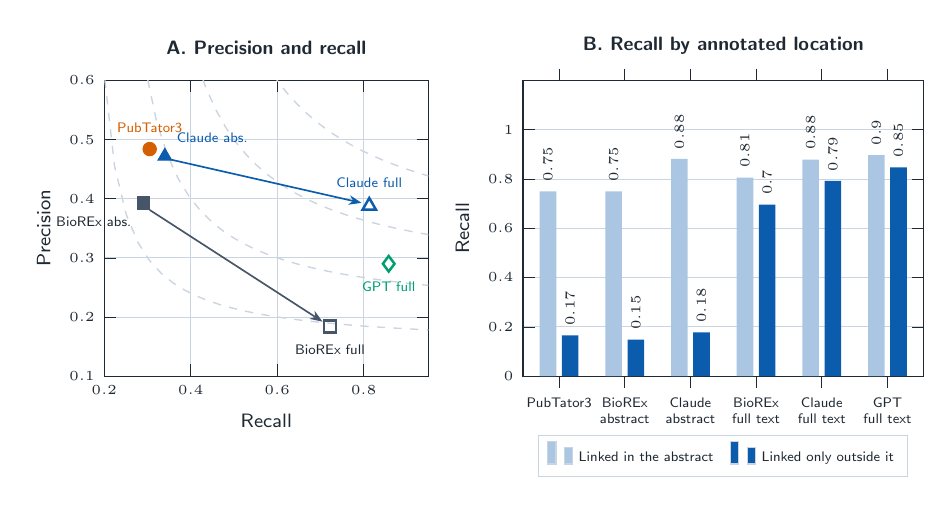
\begin{tikzpicture}
\begin{axis}[
  gdt, name=A,
  title={A. Precision and recall},
  width=0.47\linewidth, height=0.44\linewidth,
  xmin=0.2, xmax=0.95, ymin=0.1, ymax=0.6,
  xtick={0.2,0.4,0.6,0.8}, ytick={0.1,0.2,0.3,0.4,0.5,0.6},
  xlabel={Recall}, ylabel={Precision},
  clip mode=individual,
]
\foreach \F in {0.3,0.4,0.5,0.6} {
  \addplot[draw=rule, line width=0.5pt, dashed, domain=\F/2+0.02:0.95, samples=30, forget plot] {\F*x/(2*x-\F)};
}
\addplot[only marks, mark=*, mark size=2.4pt, color=pubtator] coordinates {(0.305,0.484)};
\addplot[only marks, mark=square*, mark size=2.2pt, color=stnf] coordinates {(0.291,0.393)};
\addplot[only marks, mark=square, mark size=2.2pt, line width=0.9pt, color=stnf] coordinates {(0.722,0.184)};
\addplot[only marks, mark=triangle*, mark size=2.8pt, color=ours] coordinates {(0.340,0.472)};
\addplot[only marks, mark=triangle, mark size=2.8pt, line width=0.9pt, color=ours] coordinates {(0.813,0.388)};
\addplot[only marks, mark=diamond, mark size=2.8pt, line width=0.9pt, color=gpt] coordinates {(0.858,0.290)};
\draw[-{Stealth[length=1.6mm]}, draw=ours, line width=0.6pt] (axis cs:0.355,0.466) -- (axis cs:0.795,0.393);
\draw[-{Stealth[length=1.6mm]}, draw=stnf, line width=0.6pt] (axis cs:0.305,0.381) -- (axis cs:0.705,0.192);
\node[font=\sffamily\tiny, text=pubtator, anchor=south] at (axis cs:0.305,0.495) {PubTator3};
\node[font=\sffamily\tiny, text=ink, anchor=north east] at (axis cs:0.285,0.385) {BioREx abs.};
\node[font=\sffamily\tiny, text=ink, anchor=north] at (axis cs:0.722,0.170) {BioREx full};
\node[font=\sffamily\tiny, text=ours, anchor=south west] at (axis cs:0.345,0.478) {Claude abs.};
\node[font=\sffamily\tiny, text=ours, anchor=south] at (axis cs:0.813,0.402) {Claude full};
\node[font=\sffamily\tiny, text=gpt, anchor=north] at (axis cs:0.858,0.275) {GPT full};
\end{axis}
\begin{axis}[
  gdt, at={(A.east)}, anchor=west, xshift=1.2cm,
  title={B. Recall by annotated location},
  ybar, bar width=6pt,
  width=0.55\linewidth, height=0.44\linewidth,
  ymin=0, ymax=1.2, ytick={0,0.2,0.4,0.6,0.8,1.0}, ylabel={Recall},
  symbolic x coords={pt,ba,ca,bf,cf,gf},
  xtick=data,
  xticklabels={PubTator3, BioREx\\abstract, Claude\\abstract, BioREx\\full text, Claude\\full text, GPT\\full text},
  xticklabel style={font=\sffamily\tiny, text=ink, align=center},
  xmajorgrids=false,
  enlarge x limits=0.11,
  legend style={font=\sffamily\tiny, text=ink, draw=rule, at={(0.5,-0.2)}, anchor=north, legend columns=2, /tikz/every even column/.append style={column sep=4pt}},
  nodes near coords={\pgfmathprintnumber[fixed, precision=2]{\pgfplotspointmeta}},
  nodes near coords style={font=\sffamily\tiny, text=ink, rotate=90, anchor=west},
]
\addplot[fill=ours!35, draw=none] coordinates {(pt,0.750) (ba,0.750) (ca,0.882) (bf,0.806) (cf,0.879) (gf,0.897)};
\addplot[fill=ours, draw=none] coordinates {(pt,0.165) (ba,0.148) (ca,0.177) (bf,0.696) (cf,0.792) (gf,0.847)};
\legend{Linked in the abstract, Linked only outside it}
\end{axis}
\end{tikzpicture}
}
\caption{\textbf{Precision--recall trade-offs across benchmarks, comparators, and stored-output operating points.} Error bars show 95\% document-level bootstrap confidence intervals; dashed grey curves denote iso-F1 contours from 0.3 to 0.8 in steps of 0.1 (panels A and B are zoomed to precision $\geq 0.5$). Connected markers trace operating points derived from a single model run by adding \st{uncertain} pairs to strict \st{supported} predictions; in panel A, the middle Test marker shows the \st{hedged\_claim}/\st{scope} routing rule selected on Train+Dev. On EU-ADR and RENET2, incomplete gold annotations penalize unlabelled valid predictions alongside false positives, so benchmark precision may underestimate true precision.}
\label{fig:pr}
\end{figure}

\subsection{Status Labels Against Graded Gold Labels}
Graded gold annotations test whether our status and source labels capture non-binary curation distinctions. On EU-ADR, our pipeline labelled all 3 gold negative (NA) pairs as \st{explicit\_negative}, whereas PubTator3 misclassified one as positive. Across the 122 positive (PA) pairs, our pipeline assigned 67 \st{supported}, 16 \st{uncertain}, 10 \st{not\_found}, and 4 \st{explicit\_negative}, while 25 involved an endpoint not recorded as a primary entity; counting \st{uncertain} pairs raised PA recall from 0.549 to 0.680 at 0.414 precision. On RENET2, where non-associated labels were assigned automatically to tool-proposed candidate pairs, 2 of our 223 \st{supported} predictions conflicted with an existing silver non-associated label. On BioRED, our study-versus-background source label matched the gold \emph{Novel} annotation on 526 of 703 recovered relations (75\%).

Reason codes within the \st{uncertain} status separated pairs that benchmark annotators label positive from those they exclude (Fig.~\ref{fig:recall}B). On BioRED Train+Dev, the proportion of \st{uncertain} pairs matching a gold relation was 82\% for \st{hedged\_claim} alone ($n=99$), 75\% for \st{hedged\_claim} + \st{scope} ($n=32$), and 62\% for \st{scope} alone ($n=113$), compared with 38\% for \st{presupposed\_only} and 6\% for \st{identity}. Routing only the first three reason-code groups to positive predictions raised held-out BioRED Test F1 from 0.542 to 0.627, increasing recall from 0.397 to 0.498 with little change in precision (0.846 vs 0.853) and zero extra model calls.

\subsection{Error Analysis}

\subsubsection{Missed Relations}
Decomposing all 930 missed BioRED gold relations shows that 59\% were extracted and judged non-supported, while 41\% were excluded by entity-scope boundaries (Fig.~\ref{fig:recall}A). In the first group (547 relations), the model extracted both endpoints as primary entities and assigned a non-supported status: 295 \st{not\_found}, 240 \st{uncertain}, and 12 \st{explicit\_negative}. In the second group (383 relations), one endpoint fell outside our primary entity scope: 131 involved disease mentions recorded as auxiliary symptoms or phenotypes, 159 involved unextracted disease mentions, and 93 involved unextracted gene mentions. Inspection of Train+Dev showed that unextracted mentions consisted primarily of multi-gene families or protein complexes (such as NF-$\kappa$B, MAPK, Wnt, and NMDA receptors), which our decision card excludes as single-gene endpoints, alongside broad disease categories such as ``cancer'', ``tumor'', and ``inflammation''. Even if every such broad gene or disease mention were extracted and judged \st{supported}, overall BioRED recall would increase by at most 4.0 and 6.6 percentage points, respectively.

Targeted re-querying on the Dev split tested whether unjudged same-sentence pairs reflected model oversight during whole-abstract extraction. Because 117 of the 155 unjudged gold relations on Train+Dev (75\%) had both entities in the same sentence, we ran two control experiments across the 71 Dev abstracts. First, prompt variant V4 required the model to emit an explicit judgment line for every co-mentioned pair; this constraint reduced recall from 0.454 to 0.403, lowered \st{supported} predictions from 153 to 133, increased precision from 0.922 to 0.947, and raised API cost by 16\%. Second, we isolated all 97 unjudged same-sentence pairs across 18 Dev abstracts and prompted the model in a dedicated request to judge each pair under the frozen card: 92 remained \st{not\_found}, 4 became \st{uncertain}, 1 became \st{explicit\_negative}, and 0 became \st{supported}, leaving precision, recall, and F1 unchanged at an added cost of USD 0.64. For these audited pairs, explicitly directing the model to each co-mentioned pair yielded no additional \st{supported} predictions and left all evaluation metrics unchanged.

\begin{figure}[!htbp]
\centering
\resizebox{\linewidth}{!}{% Figure 4. Where full-text predictions fall against BioTriplex (A) and the blinded checks of two categories (B).
% A: 25 articles valid for both systems, experiments/biorex/README.md. B: experiments/biotriplex/precision_check,
% precision_compare and scope_check (result.json); V6 unannotated pairs pool both checks (33 of 35).
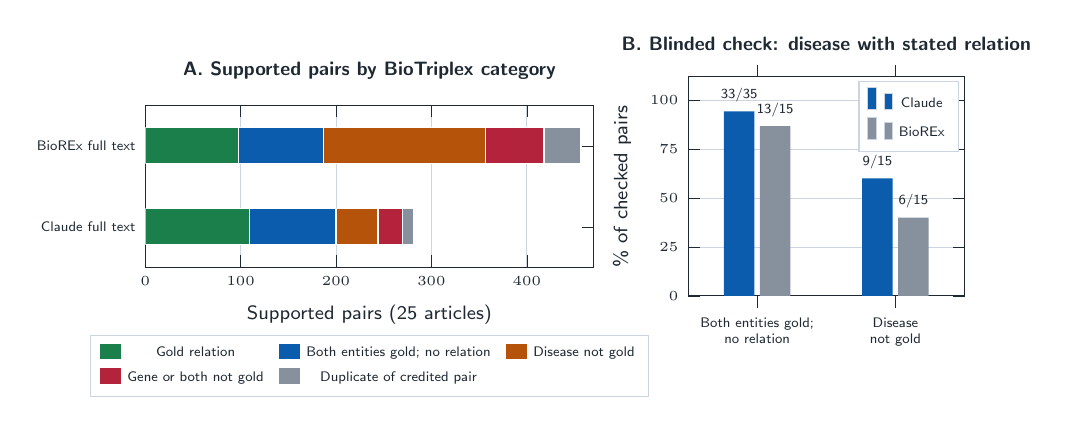
\begin{tikzpicture}
\begin{axis}[
  gdt, name=A,
  title={A. Supported pairs by BioTriplex category},
  xbar stacked, bar width=13pt,
  width=0.60\linewidth, height=0.30\linewidth,
  xmin=0, xmax=470, xtick={0,100,200,300,400}, xlabel={Supported pairs (25 articles)},
  symbolic y coords={BioREx,Claude},
  ytick=data, y dir=reverse,
  yticklabels={BioREx full text, Claude full text},
  yticklabel style={font=\sffamily\tiny, text=ink},
  ymajorgrids=false, enlarge y limits=0.5,
  legend style={font=\sffamily\tiny, text=ink, draw=rule, at={(0.5,-0.42)}, anchor=north, legend columns=3, /tikz/every even column/.append style={column sep=3pt}},
  reverse legend=false,
]
\addplot[fill=stsup, draw=white] coordinates {(98,BioREx) (109,Claude)};
\addplot[fill=ours, draw=white] coordinates {(89,BioREx) (91,Claude)};
\addplot[fill=stunc, draw=white] coordinates {(170,BioREx) (44,Claude)};
\addplot[fill=stneg, draw=white] coordinates {(61,BioREx) (26,Claude)};
\addplot[fill=stnf!65, draw=white] coordinates {(38,BioREx) (11,Claude)};
\legend{Gold relation, Both entities gold; no relation, Disease not gold, Gene or both not gold, Duplicate of credited pair}
\end{axis}
\begin{axis}[
  gdt, at={(A.east)}, anchor=west, xshift=1.2cm,
  title={B. Blinded check: disease with stated relation},
  ybar, bar width=11pt,
  width=0.42\linewidth, height=0.36\linewidth,
  ymin=0, ymax=112, ytick={0,25,50,75,100}, ylabel={\% of checked pairs},
  symbolic x coords={un,dis},
  xtick=data,
  xticklabels={Both entities gold;\\no relation, Disease\\not gold},
  xticklabel style={font=\sffamily\tiny, text=ink, align=center},
  xmajorgrids=false, enlarge x limits=0.5,
  legend style={font=\sffamily\tiny, text=ink, draw=rule, at={(0.98,0.98)}, anchor=north east},
  point meta=explicit symbolic,
  nodes near coords, nodes near coords style={font=\sffamily\tiny, text=ink},
]
\addplot[fill=ours, draw=none] coordinates {(un,94.3)[33/35] (dis,60.0)[9/15]};
\addplot[fill=stnf!65, draw=none] coordinates {(un,86.7)[13/15] (dis,40.0)[6/15]};
\legend{Claude, BioREx}
\end{axis}
\end{tikzpicture}
}
\caption{\textbf{Decomposition of missed BioRED gold relations and precision of \st{uncertain} reason codes.} (A)~Breakdown of all 930 BioRED gold relations missed under the strict view (across 419 abstracts) into pairs whose endpoints were extracted and judged non-supported (547 pairs, 59\%) versus pairs excluded by primary entity-scope boundaries (383 pairs, 41\%). (B)~Percentage of \st{uncertain} predictions on BioRED Train+Dev that match a gold positive relation, stratified by reason code. Routing pairs with \st{hedged\_claim} and/or \st{scope} reasons (blue bars) to positive predictions raised held-out Test F1 from 0.542 to 0.627 without additional model calls.}
\label{fig:recall}
\end{figure}

\subsubsection{Extra Predictions}
Partitioning \st{supported} predictions outside the gold positive sets shows that most extra predictions involve unannotated candidate pairs or background citations, with very few explicit negative contradictions. On BioRED, the 87 extra predictions split into three structural buckets: 60 cases where BioRED annotated both concepts in the abstract without a relation label, 23 cases where our disease endpoint (such as a clinical outcome) was not annotated as a BioRED disease concept, and 4 cases where our gene endpoint did not match a BioRED gene concept. On EU-ADR, 10 of our 37 extra predictions between gold concepts had been marked positive by one human annotator, falling short of the multi-annotator consensus threshold. On RENET2, among 152 \st{supported} predictions outside the gold positive set, external benchmark records show that 105 had never been inspected because no baseline tool proposed them, 45 involved an entity outside RENET2's concept vocabulary, and 2 contradicted a silver non-associated label. Within our pipeline's own provenance tags, 136 of these 152 extra RENET2 predictions were labelled \st{background}; measured precision against RENET2's gold set was 0.53 for predictions tagged \st{this study} versus 0.28 for predictions tagged \st{background}, consistent with RENET2's focus on primary study findings.

\subsection{Full-Text Extraction and Cost}
Within our pipeline on the 100-paper unlabelled PMC corpus, reading the full article body yielded nine times as many positive relation predictions (\st{supported}) as the abstract alone. Across the 100 articles, the pipeline produced 972 \st{supported} predictions, 451 \st{uncertain} pairs, and 47 \st{explicit\_negative} pairs: only 97 \st{supported} predictions (10\%) had supporting evidence in the abstract, whereas 875 (90\%) were supported exclusively by sentences in the article body. For external reference, abstract-only PubTator3 reported 198 relations across the same 100 papers; because this corpus lacks gold annotations, these counts compare candidate output volume across text scopes, not verified precision. Twenty-five papers produced zero \st{supported} predictions: 8 contained no gene mentions, 8 contained no disease mentions, and 9 contained only co-occurrences, diagnostic gene-panel lists, or speculative statements. Including validation repair calls at list API prices, extraction cost USD 0.056 per BioRED abstract, USD 4.75 across the 100 EU-ADR abstracts, USD 6.36 across the 40 RENET2 articles, and USD 0.44 per full-text article, with a mean generation time of 78\,s per full text.

%% ===================================================================
\section{Discussion}

\subsection{Why the Benchmarks Disagree}
Differences in how each corpus defines and labels relations, alongside differences in text scope and domain difficulty, contribute to the cross-benchmark F1 spread. Although the exact same frozen pipeline was applied without modification, strict F1 ranged from 0.581 on BioRED to 0.506 on EU-ADR and 0.342 on RENET2. BioRED annotates all stated abstract relations, including hedged claims, and groups symptoms, phenotypes, and broad terms such as ``cancer'' under its disease category; EU-ADR retains only relations endorsed by multiple annotators; and RENET2 labels only candidate pairs proposed by text-mining tools on longer full-text passages while assigning negative labels automatically without manual verification. A rule-governed extractor is therefore scored differently under each protocol, in addition to facing longer texts in RENET2. On incomplete gold sets such as EU-ADR and RENET2, benchmark precision penalizes valid unannotated predictions alongside genuine errors and may therefore underestimate true precision~\cite{wadhwa2023revisiting,fan2024evaluating}. Descriptive checks against the existing benchmark annotations show that many extra predictions fell into uninspected or boundary categories: single-annotator positives on EU-ADR (10 of 37) and candidate pairs never inspected by RENET2's baseline tools (105 of 152), with 0 of 3 negative pairs matched on EU-ADR and 2 of 223 \st{supported} predictions conflicting with a tool-assigned negative label on RENET2; in addition, our pipeline tagged 136 of the 152 extra RENET2 predictions as \st{background}. Because model-assigned provenance tags and non-contradiction with partial or tool-assigned negative labels do not independently prove that unannotated predictions are factually correct, formal dual-annotator adjudication remains necessary to establish true precision on these corpora.

\subsection{Implications for Curation}
Graded statuses and reason codes allow a single extraction pass to support different curation thresholds without re-running the model. An automated knowledge-base pipeline can ingest \st{supported} pairs directly while routing \st{uncertain} pairs tagged \st{hedged\_claim} or \st{scope} to human curators; on held-out BioRED Test abstracts, this deterministic post-hoc routing rule recovered 10.1 percentage points of recall (0.397 to 0.498) with a 0.7-percentage-point decrease in precision (0.846 vs 0.853). Standard binary classifiers, by contrast, conflate hedged scientific claims with entity-identity ambiguities unless retrained.

Rule-guided language model extraction and supervised classifiers play complementary roles in literature curation. PubTator3 achieves higher recall within its BioRED training domain, whereas our pipeline provides sentence-grounded records across the full text. On the BioRED test sample, combining both systems recovered 73\% of gold relations compared with 65\% for PubTator3 alone, motivating a hybrid architecture in which a fast supervised extractor proposes candidate pairs and our pipeline verifies each candidate with sentence-level evidence. Because the decision card is a version-controlled text specification, adapting the pipeline to a new relation type (such as chemical--disease associations) can begin by editing this one-page document, followed by task-specific evaluation. Close agreement between Claude Opus 5.5 and GPT-6.1 Sol under the same pipeline (F1 0.551 vs 0.555; 0.986 status agreement on full texts) demonstrates cross-model consistency across two distinct model families, although a minimal-prompt ablation remains necessary to separate the contribution of the written decision card from that of the shared output format and validator.

\subsection{Limitations}\label{sec:limitations}
Six methodological and empirical limitations bound our conclusions. First, our deterministic validator guarantees verbatim entity grounding, valid sentence-ID resolution, and schema compliance, but it does not independently verify that a cited sentence semantically proves the relation, and we have not yet conducted dual-annotator adjudication of extra predictions or missed relations; our structural breakdown of apparent false positives and re-queried misses therefore does not replace formal manual review. Second, we have not yet evaluated a minimal-prompt baseline without the decision card, leaving the relative contributions of the written rules, output format, and base model to be isolated in future work. Third, the RENET2 evaluation (40 articles) and the cross-model BioRED comparison (50 abstracts) used moderate sample sizes, producing wide confidence intervals on several metrics, and we did not perform paired significance tests. Fourth, entities are aligned by verbatim character spans without normalization to NCBI Gene or MeSH identifiers, which currently prevents cross-document aggregation and direct comparison with DisGeNET~\cite{pinero2020disgenet} or CTD~\cite{davis2023ctd}. Fifth, both Claude Opus 5.5 and GPT-6.1 Sol are proprietary models subject to version changes (we have not yet evaluated open-weight models), and public benchmark texts may overlap with pretraining corpora, just as BioRED was used to train PubTator3; to support reproducibility, we archive all prompts, raw model outputs, and evaluation scripts. Finally, each benchmark configuration was executed once (with development runs showing 0.976--0.985 pair-status agreement), our 100-paper full-text corpus lacks gold annotations to measure full-text precision and recall directly, and the released RENET2 texts are truncated to the early body.

%% ===================================================================
\section{Conclusions}
Combining a frozen one-page decision card with sentence-ID citations and deterministic validation enables gene--disease extraction from abstracts and full texts in one extraction request per paper (plus at most one validation repair call), providing deterministically grounded sentence citations, four-way certainty statuses, and provenance labels at USD 0.056 per abstract and USD 0.44 per full text. Evaluated without tuning across three benchmarks, the pipeline achieved 0.894 strict precision on BioRED, labelled all three negative gold pairs on EU-ADR as \st{explicit\_negative}, exceeded abstract-only PubTator3 recall on RENET2 full texts (0.370 vs 0.254), and showed close cross-model agreement between Claude Opus 5.5 and GPT-6.1 Sol (F1 0.551 vs 0.555). Re-querying unjudged same-sentence pairs under the same card produced zero additional supported predictions, whereas deterministically routing stored \st{uncertain} predictions by reason code recovered 10.1 recall points on held-out Test data with little change in precision (0.846 vs 0.853) and no extra model calls. Future work will complete a minimal-prompt ablation, evaluation of open-weight models, dual-annotator adjudication of extra predictions and full-text articles, concept normalization to NCBI Gene and MeSH, and hybrid curation workflows pairing supervised candidate generation with language-model verification.

%% ===================================================================
\section*{CRediT authorship contribution statement}
\todo{to be agreed with co-authors}

\section*{Declaration of competing interest}
\todo{to complete}

\section*{Data and code availability}
Code, the decision card, prompts, raw model outputs and scoring scripts will be released at \todo{repository URL}. EU-ADR and RENET2 texts are not redistributed; download scripts are provided.

\section*{Declaration of generative AI use}
\todo{Required by the publisher. Describe the use of AI tools in drafting this manuscript; check the current Elsevier wording.}

\section*{Acknowledgements}
\todo{funding and acknowledgements}

\bibliographystyle{elsarticle-num}
\bibliography{refs}

\end{document}
